\section{\textit{Function Points} approach}
\paragraph{}With this quantitative technique we can estimate the \textit{project size} in terms of \textit{function points}.\\
Function points are a unit of measure of software size, and they are used to estimate the complexity (in terms of \textit{functionalities}) of a software to be implemented, independently of the technology that will be used to implement it.

\paragraph{}Since we are interested in the \textit{functionalities} of our software, we reference directly to our Requirements Analysis and Specification Document (RASD) in order to retrieve them.

\subsection{Short description of FP}
\paragraph{}The counting of function points is based of a combination of different characteristic of the software, both internal (regarding the internal structure of the software) and external (reqarding the interaction of the system with the user or other systems).\\
With this in mind we can classify the following types of function points
\begin{itemize}
	\item \textit{Internal logic file} (ILF): the data managed internally by the application
	\item \textit{External interface file} (EIF): data used by the application but generated/maintained by other applications
	\item \textit{External input} (EI): elaboration of data coming from the external environment
	\item \textit{External output} (EO): generation of data for the external environment
	\item \textit{External inquiry} (EQ): input/output operation that do not need significant elaboration of data from the ILF
\end{itemize}

\paragraph{} We will use the following table (\ref{fp:weightTable}) in order to retrieve the \textit{weights} for each function type in the \{\textit{Simple,Medium,Complex}\} case
\begin{figure}[H]
	\centering
	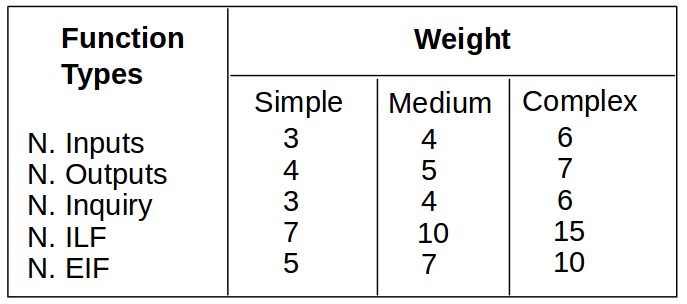
\includegraphics[scale = 0.5]{Size_Cost_Effort/fp_table}
	\caption{Function points weight table}
	\label{fp:weightTable}
\end{figure}

\subsection{Calculation for \textit{myTaxiService}}

\begin{table}[H]
\centering
\begin{tabular}{ l | c | p{0.6\textwidth} }
\textbf{ILF} & \textbf{Complexity} & \textbf{Rationale} \\ \hline
Requests & Simple & The requests of a passenger are to be stored, and they present a very simple structure (name of passenger, date of execution, location, ecc...) \\ \hline
Reservations & Simple & Similar to requests with some more attributes \\ \hline
Passenger accounts & Medium & Managing of all the data of a passenger account \\ \hline
TaxiDriver accounts & Simple & The accounts of taxi drivers are much simpler than the one of passengers. They consist simply in a username and password and the id of the taxi. \\ \hline
Taxi zones & Complex & The representation of taxi zone implies some geometry a probably the files containing them will be pretty complex \\ \hline
Taxi Queue & Medium & A taxi queue is composed by a taxi zone and the set of available taxi drivers that are in it. \\ \hline
\textbf{Total FP} & \multicolumn{2}{c}{\textbf{56}}
\end{tabular}
\caption{ILF calculation}
\end{table}

\begin{table}[H]
\centering
\begin{tabular}{ l | c | p{0.6\textwidth} }
\textbf{EIF} & \textbf{Complexity} & \textbf{Rationale} \\ \hline
GoogleMaps API & Medium & The system uses the external service offered by Google in order to parse the locations and to transform them into geographic/geometric objects. This task is estimated not to be trivial\\ \hline
\textbf{Total FP} & \multicolumn{2}{c}{\textbf{7}}
\end{tabular}
\caption{EIF calculation}
\end{table}

\begin{table}[H]
\centering
\begin{tabular}{ p{0.26\textwidth} | c | p{0.6\textwidth} }
\textbf{External Input} & \textbf{Complexity} & \textbf{Rationale} \\ \hline
Login of passenger & Simple & From the requirements\\  \hline
Logout of passenger & Simple & "" \\ \hline
Registration of a passenger & Simple & "" \\ \hline
Deletion of passenger account & Medium & Differently from the other basic operations on the account of a passenger, this one involves the elimination of all the requests and reservations. \\ \hline
Login of taxidriver & Simple & From the requirements \\  \hline
Logout of taxidriver & Simple & "" \\ \hline
Make a request & Medium & Not an easy operation: it involves the storing of the request, the validation of the input and the parsing of the locations, ecc... \\ \hline
Make a reservation & Complex & This operation involves a lot of components in our system and probably is the most demanding one. \\ \hline
Setting of availability of taxi driver & Medium & It involves the setting of the zone and the pop/push into a taxi queue \\ \hline
Accepting/Refusing a ride & Medium & It involves the re-forwarding of the request/reservation and the notification to the passenger in case of problems. \\ \hline
\textbf{Total FP} & \multicolumn{2}{c}{\textbf{37}}
\end{tabular}
\caption{External Input calculation}
\end{table}

\begin{table}[H]
\centering
\begin{tabular}{ p{0.26\textwidth} | c | p{0.6\textwidth} }
\textbf{External Output} & \textbf{Complexity} & \textbf{Rationale} \\ \hline
Sending of a request of a ride to a taxi driver & Medium & We need to retrieve the correct taxi driver and send him all the data regarding the ride \\ \hline
Acknowledgment of reservation to a passenger & Simple & It only require the generation of a string on the base of the outcome of the reservation process. \\ \hline
Sending to the passenger the meeting data of a request & Medium & It involves the calculation of the estimated waiting time \\ \hline
\textbf{Total FP} & \multicolumn{2}{c}{\textbf{14}}
\end{tabular}
\caption{External Output calculation}
\end{table}

\begin{table}[H]
\centering
\begin{tabular}{ p{0.26\textwidth} | c | p{0.6\textwidth} }
\textbf{External Inquiry} & \textbf{Complexity} & \textbf{Rationale} \\ \hline
Visualize the list of reservations of a passenger & Simple & From the requirements \\ \hline
\textbf{Total FP} & \multicolumn{2}{c}{\textbf{3}}
\end{tabular}
\caption{External Inquiry calculation}
\end{table}
Finally we do a resume, calculating the total number of function points.
\begin{table}[H]
\centering
\begin{tabular}{ l | c }
\textbf{FP type} & \textbf{Number of FP} \\ \hline
ILF & 56 \\ \hline
EIF & 7 \\ \hline
External Input & 37 \\ \hline
External Output & 14 \\ \hline
External Inquiry & 3 \\ \hline
{\large \textbf{Total FP}} & {\large \textbf{117}}
\end{tabular}
\end{table}
